\chapter{Required Background Knowledge}
\label{ch:background}

This chapter provides the background information needed to understand the chapters that follow.  It examines the basic outline of a communication system and how non-idealities are compensated for, with the addition of multiple input multiple output (MIMO) systems and a unique filtering technique called spectral subtraction.   Secondly, this chapter investigates common jammer scenarios and anti-jamming solutions.  Finally, it outlines the necessary hardware and software tools used in the implementation chapter.

\section{Jamming}

In 1899 Guglielmo Marconi successfully transmitted radio messages across the English Channel, and nine months later Alexander Bell was discussing how this could be jammed during wartime \cite{10}. Bell stated that such a wireless system can be easily disrupted with simple electromagnetic distrubances:  ``It's as easy as cutting the wires'' \cite{10}.  In the early days of wireless communication, such systems were very fragile but today they have become substantially more resilient. In its simpliest form, radio jamming is the transmission of electromagnetic signals that interfere with communications by decreasing the signal to noise ratio (SNR) between the transmitter and receiver.  This jamming can be either deliberate or unintentional, and can either entirely disable the communication link or limit its capacity.  , a common example of unintentional jamming is microwave ovens which operate at a wavelength of 122 millimetres which translates to 2.45GHz from this equation: \(\lambda=\frac{v}{f}\), with \(lambda\) representing the wavelength, \(v\) the velocity and \(f\) the frequency. This band directly interferes with channels defined under the IEEE 802.11 standard, also known as Wi-Fi \cite{ieee80211}.  Deliberate jamming on the otherhand, is generally more saphisticated and takes many different forms.\\

Intentional communications jamming is usually aimed at radio signals in a combat setting, where consequences are insigificant or out of the relm of the law. In the most rudimentary designs, a jammer will simply tune their own frequency to that of their opponent and with a similar moduation scheme (and significant power) disrupt the enemies transmissions.  The most common types of this form of signal jamming are: random pulses, stepped tones, warbler, tones, rotary, pulses, sparks, recorded sounds, gulls, sweep-through, and random noise \cite{sterling}.  These methods obviously (or subtly) disrupt transmissions by inserting electronmagnetic energy into the transmission space of the receiver.  In more technical terms, the jammer is producing randomly chosen data that is non-orthogonal to the data which the friendly transmitter is producing.  Since this jammer's data is pseudo-random when his transmissions are added to the `oponent's' signal, the result appears to be random as well.  Therefore, the signal is unrecoverable.  As mentioned above, the jammer must produce signals that are non-orthogonal to the enemy of his jamming will have no effect.  An example below shows random noise at a significant noise level is added to a previously destinquishable signal.\\

\begin{figure}[!ht]
  \begin{minipage}[b]{0.5\linewidth}
    \centering
    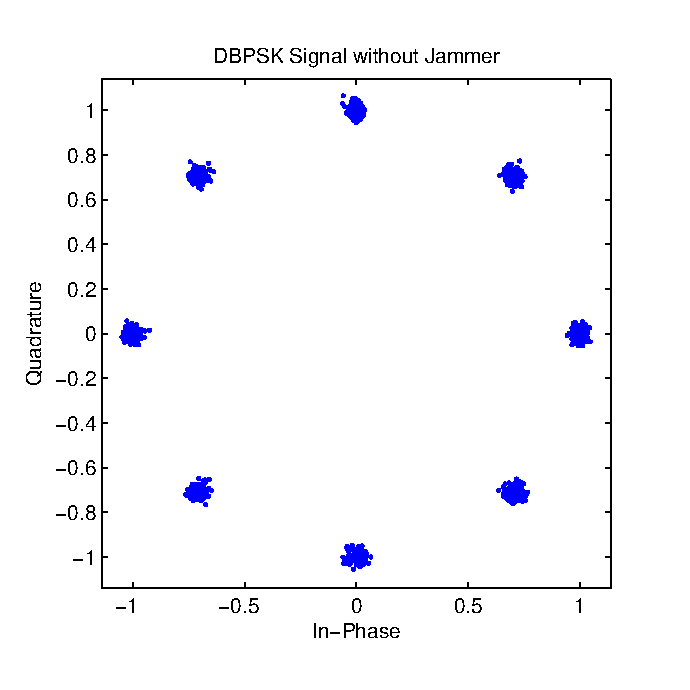
\includegraphics[width=\linewidth]{DBPSK_nojam.eps}
    \caption{DBPSK signal uncorrupted by jammer.  Clean clustering around the constellation points provides accurate symbol recovery.}
    \label{fig:chapter001_dist_001}
  \end{minipage}
  \hspace{0.5cm}
  \begin{minipage}[b]{0.5\linewidth}
    \centering
    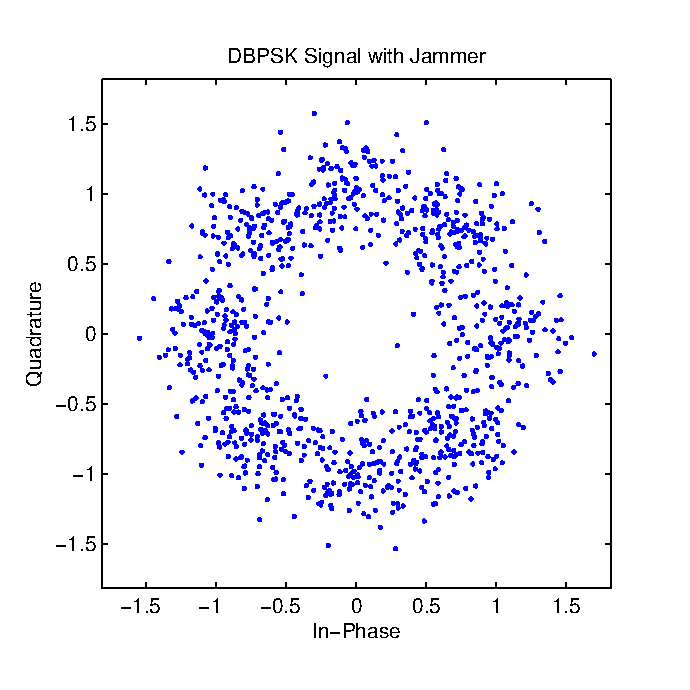
\includegraphics[width=\linewidth]{DBPSK_jam.eps}
    \caption{DBPSK signal corrupted by jammer.  The overlapping clustering around the constellation points provides difficult symbol recovery.}
    \label{fig:chapter001_reward_001}
  \end{minipage}
\end{figure}

\section{Anti-Jamming}

Anti-jamming has been considerably outlined in the Introduction chapter, therefore this section will examine more advanced narrowband and wideband techniques that involve filtering rather than avoidance.  All of these approaches have various monitary costs, constraints, and power limitations.  First, narrowband mitigation techniques will be considered.  These include adaptive filtering, time-frequency domain filtering, adaptive antennas and subspace processing.  By combining several of the listed techniques, wideband jammers can also be address, under certain conditions.  Table \ref{antitable} compares these techniques with various attributes.\\

\begin{table}[!ht]\label{antitable}
\centering
\caption{Comparision of Anti-Jamming Techniques}
\resizebox{\columnwidth}{!}{
    \begin{tabular}{|l|l|l|l|l|l|}
        \hline
        Technique                       & Cost & Size  & Flexibility                              & Complexity  \\ \hline
        Adaptive Filtering              & low  & small & ~                                        & ~           \\ 
        Time-Frequency Domain Filtering & ~    & ~     & ~                                        & ~           \\ 
        STFT                            & low  & small & Environment Specific                     & low         \\ 
        Filter Banks                    & low  & small & Environment Specific                     & low         \\ 
        Wavelet Transform               & low  & small & Environment Specific/Resolution Required & low         \\ 
        Subspace Processing             & low  & small & ~                                        & ~           \\ 
        Adaptive Antennas               & ~    & ~     & ~                                        & ~           \\ 
        Null Steering                   & high & large & ~                                        & high        \\ 
        Beam Forming                    & high & large & ~                                        & high        \\
        \hline
    \end{tabular}
}

\end{table}

Adaptive filtering is a well defined solution in jammer mitigation, but it is to date the most limited.  Most notably, the jammer must be a relatively narrowband and the period of the jammer must be relatively short.  An example of an adaptive filtering technique is a suppression filter.  Suppression filters assume statistically the signal is Gaussian, which results in the optimal filter being linear.  This filter essentially solves the Wiener equation for an optimal filter, but generally a Least Mean Square (LMS) implementation is used instead of just inversing the channel estimate \cite{11}. The technique of inverting the channel estimate or correlation matrix is traditionally called a zero forcing equalizer and is extremely unstable in the presence of small noise.\\

Next, time-frequency domain filtering attempts to represent the transform the received signal in such a way that it is possible to easily distinguish the jammer from the data signal.  A Short-Time Fourier Transform (STFT) can be used to accomplish this goal.  A STFT operates by sliding a window across a signal and taking the fast fourier transform (FFT) of that window. Reference \cite{12} uses the STFT to break a signal into its frequency components. From this information, with a narrowband jammer only a small number of frequency domain bins contain nearly all of the interferers.  Therefore these bins can be simply nulled and an inverse FFT can be applied to the signal to regain its time domain version.  This is very effective with the use of a spread spectrum signal with a narrowband jammer.\\

%\being{equation}
%
%\displaystyle\sum_{n=-\infinity}^{\infinity} n^{2}
%
%\end{equation}

Filter banks is a second methodology that can be used to reduce spectral leakage in the frequency domain, which is the primary drawback with the STFT approach.  One advantage of the filter banks approach is they do not inject interference when the jammer is not present, which is a common problem when the jammer turns on and off frequently.  Filter banks provide jammer suppression after their spectral decomposition stage, since at this point sub-band encoding can be accomplished this spectral modification simply nullifys the jammer \cite{13}.  A similar decomposition is the wavelet transform.  Unlike the STFT, the wavelet transform is much more flexible because the STFT has a fixed resolution for a given FFT size unlike the wavelet transform \cite{wavelet}.  Subspace processing which is a form of wavelet transform, is applied in this way.  The jammer subspace can be made orthogonal to the wanted signal subspace, nullifying the jammer's effects \cite{14}.\\

Besides these signal processing methods, physical techniques can also be use to do spatial filtering.  These techiques make use of several antennas, and as an assumption the number of interferers must be equal to or less than the number of antennas.  The first approach is called Null Steering.  Null Steering constantly computes the weights in order to minimize the received energy level. In effect, this technique attempts to steer the antenna away from the jammer.  The second approach is called Beamforming.  Beamforming tries to adjust the antenna in order to maximize the SNR. In effect, the antenna beam is steered in the direction of the desired signal.  It is of course, possible for the jammer's signal to be in the same direction as the signal source. Therefore the postcorrelation technique is used in order to obtain the SNR. However, prior knowledge of the signal direction and the host location is required \cite{kandangath}.  It is also important to note that larger the number of elements in the array itself, the closer the jammer can physically be located to the desired transmitter.\\


Historically, all of these approaches historically were applied to spread spectrum communication systems because narrowband jammers fundamentally are considerably easier to deal with in this setting.  They are more straightforward because the jammer effects only a fraction of the transmitter's transmission space; therefore, when wideband jammers exist many of these schemes fall apart.  Other avenues or scenarios must be considered in such situations to overcome this limitation.  Before a solution is chosen, additional signal processing and communication theory must be understood.  These topics will be examined in the following sections.\\



\section{Communication Systems}

Modern wireless digital communication systems are based on a rich tradition of analog experimentation and theory.  These signal technologies surround us constantly, such as cellphones, car radios, GPS, and more.  All these of these devices communicate over wireless links and are built upon the same building block of transmission and reception theory.  Many perspectives can be taken, but a more generic observation should be taken at the system level.  Depending on the level of sophistication these blocks can expand greatly, but still solve the same issue caused by the wireless transmission of digital access across their environment.  Such non-idealities such as frequency offsets, doppler effect, signal echoes, phase shifts, and others must be compensated for to successful receive uncorrupted information.\\ 

Let us examine the transmitter first since it is less complicated than the receiver.  The transmitter's primary goal is to send data in a resilient form, or structure, to create a more managable signal for the receiver.  This is accomplished in several steps, and the function, or purpose, of the overall system determines the sophistication of the design.  Figure \ref{fig:Transmitter_System_Diagram} outlines the major building blocks of the transmitter; consisting of the coder, pulse-shape filter, and frequency translator.  A filter is added after the coding block in some implementations to provide such effect as pre-distortion.\\

\begin{figure}[!ht]\label{fig:Transmitter_System_Diagram}
\centering
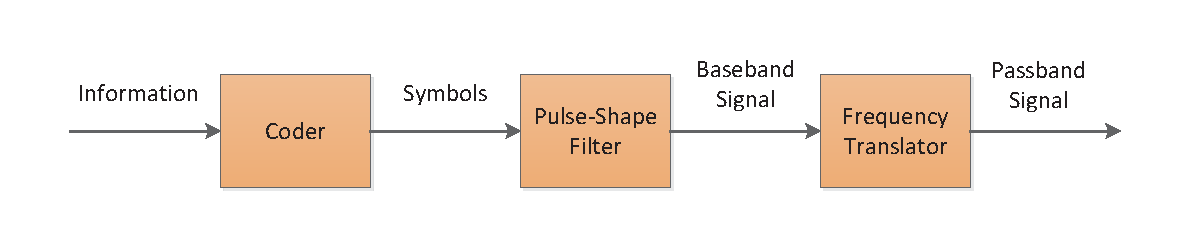
\includegraphics[scale=0.8]{Transmitter.eps}
\caption{Basic transmitter outline, converting information or data to a easily recoverable signal by the receiver.}
\end{figure}

The transmitter's sole purpose is the send data that is convenient for the receiver to understand, and allow others to use the transmission medium as well.  The coding phase of the transmitter can have many features and purposes, but simply it will encode data into a symbol with a form of redundancy or scheme that will help the receiver reconstructed the information more easily.  Next the pulse-shape filter is used to help separate data and help maximize the SNR at the receiver.  This filtering can be done with an assortment of filter shapes, but the most popular is the raised square-root cosine filter.  After pulse-shaping, the signal is translated into frequency information and unconverted to a high RF with a carrier signal.  The translation is done with a modulation scheme such a binary phase-shift keying (BPSK) or pulse amplitude modulation (PAM).  The is up-converted by mixing the signal with a sinusoid, seen by Equation \eqref{mixing}.

\begin{equation}[!ht]\label{mixing}
cos(x)cos(y)=\frac{(cos(x+y)+cos(x-y))}{2}
\end{equation}

This done because low-frequency signals such as speech, music, or digital data can be much more efficiently transmitted at higher frequencies \cite{9}.\\

Now let us discuss the receiver.  At the system level, a modern digital receiver can be broken down into a small set of distinct categories or operations: carrier synchronization, timing synchronization, equalization, and frame synchronization, as outlined in Figure \ref{Receiver_Blocks}.  These sections work together in series to provide smooth transmission of data, and many techniques exist within theses categories to accomplish its goal.  In most communication systems, after the radio frequency (RF) front-end, the first operation done on the received signal is frequency compensation and down conversion.  This compensation needs to accomplished because non-idealities and differences exist between the transmitter's and receiver's oscillator.  Therefore this is continually compensated for and corrected.  Carrier recovery can be accomplished using several methods that include but are not limited to: squared difference loops, phase-locked loops, costas loops, and decision-directed phase tracking \cite{9}.\\

\begin{figure}[!ht]\label{Receiver_Blocks}
\centering
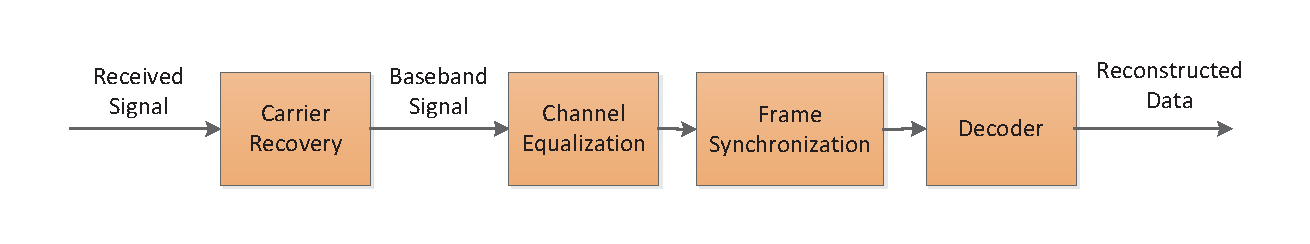
\includegraphics[scale=0.7]{Receiver.eps}
\caption{Basic wireless receiver outline, with four primary blocks.  All designed to remove corruption caused by the wireless environment and translate transmitted signals back to desired data.}
\end{figure}

After carrier recovery, the signal is pulse-shaped with the same filter shape used at the transmitter.  This technique will help to maximize the SNR of the signal.  Then the signal must be corrected again for timing.  The purpose of timing recovery is to choose the instants at which to sample the incoming signal.  This is generally done through a interpolation mechanism of the transmitted signal.  Since at the transmitter the signal is upsampled to symbols, a single data point or bit is represented by several received data points.  Therefore these points can be interpolated together for a more accurate estimate of the original data.  Timing recovery also can be done with one of several methods including: output power maximization, Mueller-Muller method, or decision-directed.  Generally, they utilize their own interpolation algorithm, such as sinc-interpolation \cite{9}.\\

After this point the receiver designs can vary greatly, as the design in this thesis will present, because this is where most of the digital signal processing (DSP) will take place.  This section, call Equalization, is responsible to correcting any effect the channel has on the signal. This includes multi-path, noise, 	and other distortions that cause inter-symbol interference (ISI).  Equalizer implementations are designed to compensate for types of disturbances that occur using certain systems.  The equalizer stage is most often coupled with the frame synchronization stage such that the equalizer itself can adapt to changing conditions.  This is known as soft decision making.  Equalizer techniques include but are not limited to: LMS , decision-directed, dispersion-minimizing \cite{9}, Viterbi \cite{viterbi}, blind, and turbo equalizers \cite{turbo}.\\  

\subsection{Equalization}

Equalizers can be considered the most complicated design of an entire communication system since they combat a series of distortions.  The primary result of these distortions is called inter-symbol interference (ISI).  ISI simply means that symbols interact with one another in the channel space and cannot be considered independent from one another.  Since this interference is generally considered a frequency selective disruption or dispersion a filter needs to be employed to reverse such effects.  This filter must be adaptable because the channel distortion cannot be know prior to transmission.\\  

As listed in the previous section, many equalizers exists and operate under specific conditions.  Here several linear equalizers will be discussed in detail including maximum-likelihood sequence detection, adaptively trained equalizer, and decision-directed linear equalization.  The goal of all of these equalizers is to find a finite impulse response (FIR) filter that when convolved with the received signal produces the original transmitted data \( \boldsymbol{\hat{X}}=\bf{Y} * \bf{G} \).  Figure \ref{FIR_filter} outlines a typical FIR structure for which the equalizer will create the appropriate coefficients \(b_{0},b_{1},..., b_{n} \).  These equalizers also examine the condition of an additive white Gaussian noise (AWGN) channel, and uncorrelated or independent interferers.\\

\begin{figure}[!ht]\label{FIR_filter}
\centering
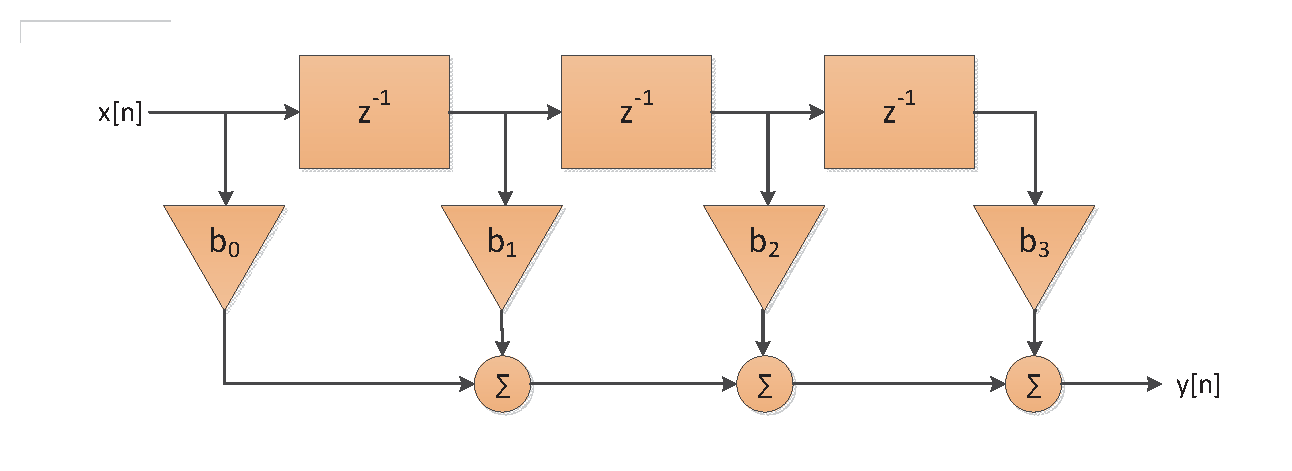
\includegraphics[scale=0.7]{FIR_filter.eps}
\caption{FIR Filter Structure}
\end{figure}

The Zero Forcing Equalizer (ZFE) uses peak distortion criteria to determine equalizer coefficients.  The ZFE produces zero ISI at its output.  If \(H_{c}(f)\) is assumed to be the effects of the channel, the ideal equalizer would be \( H_{eq}(f)=\frac{1}{H_{c}(f)}\).  This can also be consider the inverse of the channel.  The filter coefficients are modeled as weighted pulses convolved with the channel, which can be expressed as Equation \eqref{weighted}.  Here \(b\) represents the weighted filter taps, \(p_{r}\) represents the input signal and \(p_{eq}\) represents the output of the filter.

\begin{equation}\label{weighted}
p_{eq}(t) = \displaystyle\sum_{k=-M}^{M} b_{k}p_{r}(t-kT)
\end{equation}

Unfortunately, the ZFE has a large disadvantage; it cannot compensate for small amounts of noise.  Technically, the ZFE will amplify all noise of the received signal, and if any elements of the channel matrix are considerably small, then the equalizer becomes unstable. Therefore this is generally considered a more theoretical or elementary equalizer formulation.  To overcome this problem the zero ISI condition must be relaxed allowing for noise which if small can easily be overcome by such operations as quantization or decision making.  The Linear Minimum Mean Squared Error Filter (LMMSE) takes this relaxation into account \cite{spinger}.\\ 

The LMMSE assumes that the symbols are uncorrelated with one another and uncorrelated from the noise in the channel.  This approach tries to minimize the mean square error, a common measure of estimator performance.  The estimator is defined as \(\hat{x}_{MMSE}(y)=E{x|y}\), where we are given the received signal \(y\) and must guess or estimate \(x\), which was transmitted originally.  If \(x\) and \(y\) are jointly Gaussian, then the LMMSE will be linear.  This function or equalizer design minimizes the mean square error.  To simplify further an extension to random vectors can be examined.  An estimate can be made for the original vector \(x\) represented by \(\hat{x}\), resulting in the linear equation \(\hat{x}=ay+b\).  \(a\) and \(b\) represent the coefficients to be selected for the estimator.  The LMMSE will minimize the mean square error shown in Equation \ref{mse}:

\begin{equation}\label{mse}
 MSE = \|x-\hat{x}\|^{2}
\end{equation}

Besides these linear equalizers outlined, an adaptive approach can also be considered.  The Least Mean Squares (LMS) or Gradient Descent algorithm utilizes a traditional technique for minimizing the error in a signal.  This method is historically known as the "Method of Steepest Decent" or a very closely related algorithm called "Newton's Method". By calculating the error of each received symbol, this can be fed back into the system for future symbols.  This error will shape the equalizer's filter coefficents to match the inverse of the channel.  The equations \ref{lms_eq}, \ref{lms_eq2}, and \ref{lms_eq3} outline the LMS algorithm.

\begin{equation}\label{lms_eq}
y[n]=w[n]^{H}u[n]\\
\end{equation}

\begin{equation}\label{lms_eq2}
e[n]=d_{n}-y[n]\\
\end{equation}

\begin{equation}\label{lms_eq3}
w[n+1]=w[n]+\mu u[n]e^{*}[n]\\ 
\end{equation}

In these equations: \(w\) represents the adaptive filter coefficients, \(u\) the input signal, and \(d\) the known signal.  \(\mu\) acts as the algorithm's step-size determining how quickly it will converge.  It must also be considered that the larger the step-size the higher the probability it may become unstable.  As long as the channel's effects are slow changing, this equalizer can easily maintain up to date estimates while corrupting as little of the data as possible.\\  

All of the methods proposed so far require \textit{known} data (\(d_{n}\) in Equation (\ref{lms_eq2}) to correct against.  This data is called training data and generally comes in the form of a preamble in a frame.  The preamble is added to the beginning of each frame so the equalizer can learn from the effects on that specific data.  The preamble is the same for all frames and is always used so the equalizer will always be learning.  However, what happens when data is unknown in the frame, such as the payload portion of the frame.  This is where blind equalization is employed.\\

Several blind equalizers exist but an extension of the LMS equalizer for blind situations will be examined here called the decision-directed equalizers \cite{9}.  For a blind equalizer to operate an error generation mechanism must be evaluated, but since the data symbols are unknown, a decision device must be used in place.  This decision device is a quantization method and the error is generated from this quantization.  This error generation is extrapolated from expression: 
\(e = \frac{1}{2}(sgn(y[k]-y[k])^{2}\)
Where the \(sgn\) function returns 1 for positive numbers and -1 for negative numbers.  This expression is quite similar to the original LMS implementation except instead of a known symbol the data is quantized using the sign function.  This type of quantization using the sign function is only applicable with binary modulation schemes such as BPSK.  This equalizer method is usually combined with a training equalizer method in practice, since if a nearly closed eye is observed, when using an eye diagram, this equalizer cannot open it by itself.  An example of such an eye diagram is shown in Figure \ref{eye_closed}, and clean/open eye diagram can be seen in Figure \ref{eye_clean}.\\

\begin{figure}\label{eye_clean}
\centering
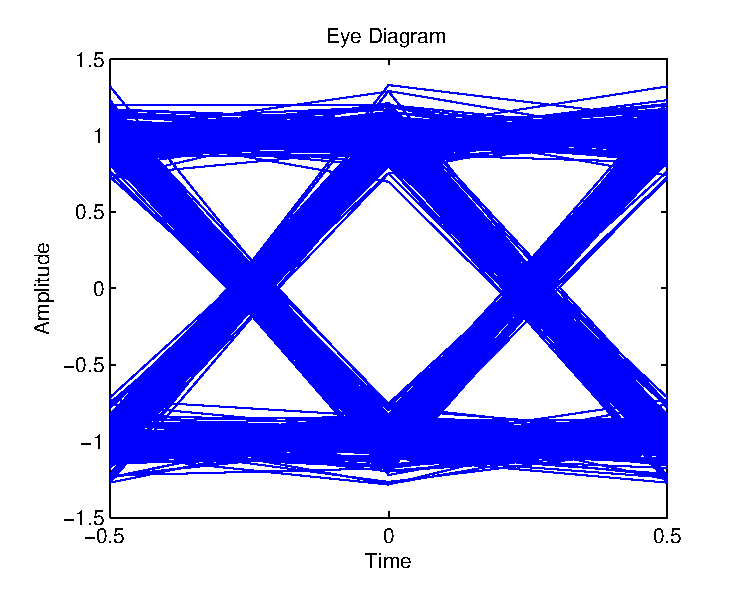
\includegraphics[scale=0.8]{eye_clean.eps}
\caption{Adequate timing recovery produces open eye, which clearly defines the received symbols in time.}
\end{figure}

\begin{figure}\label{eye_closed}
\centering
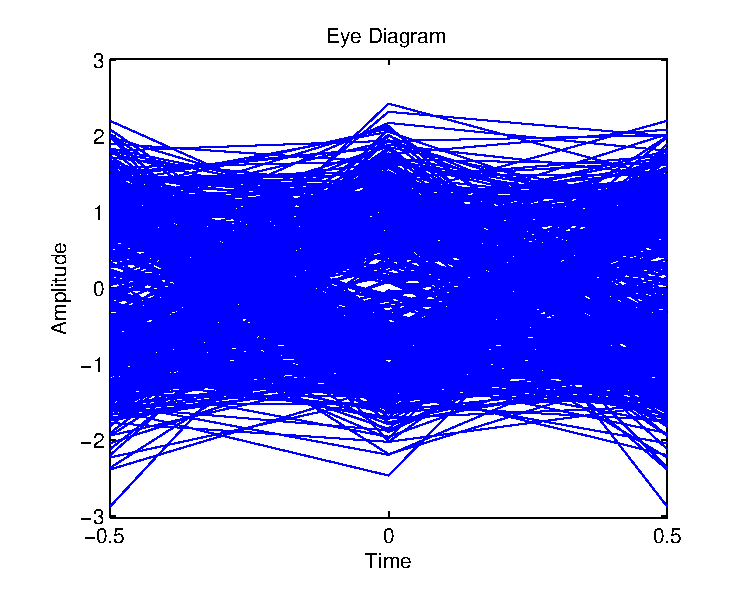
\includegraphics[scale=0.8]{eye_closed.eps}
\caption{Poor timing recovery produces a closed eye, identifying that the signal cannot be recovered unless corrective measures applied.}
\end{figure}

In this section, we have examined several equalizer techniques while outlining their advantages and disadvantages.  Most techniques require some training mechanisms to operate under heavy channel distortion, and blind techniques such as decision-directed equalization will fail under these conditions.  Unfortunately, such training data can take considerable resources, and lower overall data throughput.  In practice as much as 20\% of frame information is training.  Therefore other techniques must be considered to help overcome this obstacle.\\


\subsection{Superimposed Training Equalization}

As mentioned in the previous section, many implementations exist for equalizer designs, but this thesis will examine the effectiveness of superimposed training symbols in frequency selective channels.  In traditional equalizers, channel estimation is achieved through the use of training data or pilot symbols.  These symbols are both known to the transmitter and receiver, providing the basis for an estimate.  In these equalizers all training symbols are placed at the start of a frame, with \cite{16} showing that under high SNR training-based schemes are capable of capturing most of the channel capacity, while under low SNR they are highly suboptimal.  Superimposed equalizers try to overcome this problem along with others to provide more optimal estimates.  Superimposed equalizers physically add training symbols to the data stream instead of concatenating symbols, saving valuable bandwidth \cite{16}.  To accommodate such pilots, energy must be shared among the data and hidden pilots \cite{Ghogho}.  Reference \cite{19} shows that for a transmitter of fixed power, with an additive pilot sequence, the decrease in data signal power is equal to: \[ K_{loss}=\frac{E[\|s(k)\|^{2}}{E[\|s(k)\|^{2}]+E[\|u(k)\|^{2}]}\] equivalent to \(10logK_{loss}dB\) in signal to noise ratio (SNR).  With \(s(k)\) representing the source signal, and \(u(k)\) representing the received signal.  Other disadvantages include an increased signal envelope fluctuation that can be undesirable in nonlinear transmit power amplifiers \cite{17}.\\  

At the receiver, channel estimation can be done using several techniques in both the frequency and time domain.  Reference \cite{17} examines a time domain approach for synchronized averaging of the received signal.  It is important to note that this synchronization is not related to transmitter and receiver synchronization.  References \cite{17} and \cite{18} both assume that the signal \( \bf{x}(n)\) and noise \( \bf{v}(n) \) have zero mean and \(E[m_{x}(n)] = \bf{d}(n) = \bf{p}(n) \ast \bf{h}(n)\).  Therefore, since \(\bf{p}(n) \) is the known superimposed periodic pilot sequence, \(\bf{h}(n)\) can be determined.  Note that \(\bf{h}(n)\) is generally considered frequency selective, and such channels can be quite difficult to deal with especially with multi-path.  Multi-path interference is a distortion caused when copies of the original signal arrive at the receiver delayed on top of the originally received non-delayed signal.  This delayed signals essentially take other paths to the receiver, and this interference's manifestation is commonly called \textit{ghosting} in such applications as television broadcasts \cite{ghost}.\\

Superimposed equalizers are able to better compensate for large multi-path channels because they can spread their training symbols throughout the signal itself.  This spreading not only provides a spreading in time but also in other dimensions such a frequency.  Therefore, if the training symbols are chosen correctly and placed correctly, they can then be spread across the frequency spectrum efficiently and capture its selectivity.  Before the pilots can be examined, the channel must be defined.  The channel is of block length \(N\), and the channel is also time invariant across single blocks, but variable across blocks.  The memory of this channel is of maximum length \(L-1\), and the impulse response of the channel is defined as \(\textbf{h}=[h_{0},...,h_{L-1}]^{T}\).  Since there are \(N\) blocks in the channel, the channel matrix \(H\) is modeled as an \(N x N\) circulant matrix, with the received signal as expressed as:

\begin{equation}
\textbf{x}=\textbf{H}\textbf{s}+\textbf{v}
\end{equation}

Here, \(\textbf{v}\) is assumed to be zero mean white noise.  The vector \(\textbf{s}\) is a combination of known training symbols and unknown data.  The optimal placement for such training is where the channel undergoes non-ergodic fading considered here \cite{20}.  Reference \cite{16} continues on to say that optimally, assuming symbols are placed in clusters of length \(\alpha \ge 2L+1\), this scheme is quasi-periodic.  The variable \(\alpha\) represents the cluster size in this scenario.  It is also important to note that this placement makes sure that the training is always orthogonal.\\

Another effect that must be considered is how these training symbols interfere with the data itself, and is the training symbols dependent on the data or even the modulation scheme.  Reference \cite{Ghogho} examines this aspect and proposes solutions that provides a data independence condition.  As explained previously, since the training data is periodic it can be placed in equispaced frequency bins, while data is spread across all frequency bins.   Therefore, the pilot must be designed to distort the data vector of the discrete Fourier transform to zero.  In the superimposed training data case, this is done by using the cyclic mean of the data.  Therefore, all that needs to be done is the removal of the cyclic mean \(\textbf{e}=\textbf{Jw}\).  Note that \(\textbf{J}\) is the Kronecker product of an identity matrix and the fractionally spaced locations of the pilot tones.  Therefore, at the pilot frequency only the training symbols are visible for the channel estimation.  Formally here is the transmitted, or precoded, result including pilots and data: \( \textbf{s}= (I-\textbf{J})\textbf{w}+\textbf{c}  \).\\


In summary, research on superimposed training focuses primarily on the training symbol generation for a certain type of communication systems design from single transmission to multiple-input multiple-output (MIMO).  Unfortunately, little to no physical implementations exists for such systems.  This is true because of the synchronization issue that exists when using superimposed training symbols.  Since they are directly placed with transmission data it can be difficult to determine their locations in a sequence blindly, which is done in real world systems.  This problem must be considered when physical implementations are proposed.\\

\section{Spectral Subtraction}

Now that methods of reconstructing information distorted by the channel itself has been discussed, we can now focus on spectral removal of known signals without demodulation.  Such a technique is needed to improve the effectiveness of equalization operations done downstream, while limiting corruption to the desired signals themselves.  In this thesis a new application for a relatively standard technique was examined, called Spectral Subtraction (SS).  The SS technique was first published in 1979 by Steven Boll \cite{boll}. SS is formally used to reduce ambient noise in audible sources, improving the overall quality and intelligibility of digitized speech.  It is a dominant speech processing algorithm and many extensions including \cite{SSEXAMPLE}, \cite{SSEXAMPLE2}, and \cite{SSEXAMPLE3}.  Due to the large amount of literature and investigation into the SS process it was assumed to be a solid option for removing unwanted signals in the spectrum.\\

SS primarily was designed for audio signal processing, small bandwidth signals roughly from 20Hz to 20,000Hz.  Many forms of SS exist, but the approach examined here is Magnitude Spectral Subtraction (MSS).  It works by first generating an estimate of the noise in the signal itself, which is usually attained at the first first few seconds of the signal itself.  This noise is then subtracted, as the name suggests, from the rest of the signal.  Mathematically, let us explain this further.  The received signal is assumed to be a combination of two signals, the transmitted and the noise itself \(y(t) = x(t) + n(t)\).  Next the power spectral densities (PSD) are calculated for these components:

\[ E\{|Y(e^{jw}|^{2}\}= E\{|X(e^{jw}|^{2}\} + E\{|N(e^{jw}|^{2}\} + 2E\{|X(e^{jw}|^{2}\}\{|N(e^{jw}|^{2}\}\]
\[ E\{|Y(e^{jw}|^{2}\}= E\{|X(e^{jw}|\} + E\{|N(e^{jw}|\}  \]

Here \(Y(e^{jw})\), \(X(e^{jw})\), and \(N(e^{jw})\) represent the frequency domain transform of the given signal, also \(x\) and \(n\) are uncorrelated.  Since at points when the desired signal is not present in the spectrum, a silent period, the measurement for \(N\) is taken and then subtracted from the entire received signal \(E\{|X(e^{jw}|\}= E\{|Y(e^{jw}|\} - E\{|N(e^{jw}|\}\).  The is noise is assumed to be quite stationary during the signal period.  Therefore, the original estimate \(\hat{N}\) can be quite accurate.\\

\subsection{Residual Noise}

As a result of the changes over time in the noise spectrum (whether power or magnitude) around its expected value, there is always some difference between the actual noise and its mean value. Hence, some of the noise remains in the spectrum in the case that the value of noise is greater than its mean and some of the speech spectrum also is removed in the case that the estimate of noise to be greater than the actual value of noise. The latter produces negative values in the spectrum. These negative values are prevented or set to a floor (sometimes zero) using different techniques. The overall effect puts noise in the output signal known as residual. The narrow band relatively long-lived portion of residual noise is sometimes referred to as musical noise \cite{mnoise}.

A close examination of musical noise, shows that peaks and valleys exist in the short term power spectrum of white noise.  These frequency locations for one frame are random and they vary randomly in frequency and amplitude from frame to frame. When a smoothed estimate of the noise spectrum is subtracted from the actual noise spectrum, all spectral peaks are shifted down while the valleys are set to zero. Therefore, after this subtraction sharp peaks remain in the noise spectrum and pre-existing ones can be sharpened. The wide peaks are generally estimated as time varying broadband noise. The narrower peaks, which are relatively large spectral distances because of the deep valleys that define them, are perceived as time varying tones which are generally referred to as musical noise \cite{berouti}.

Therefore, \cite{boll} continues by introducing a ``smoothing'' technique before the signal is convert back into the frequency domain.  Two additional parameters are introduced: The parameter \( \alpha \) the over-subtraction coefficient, and \(\beta\) the noise floor lower bound.  \(\alpha\) is used to provide a more aggressive subtraction to the signal, attacking high peaks which are generally a result of high noise and an inaccurate initial estimate.  The second parameter \(\beta\) is used to fill in the valleys of the signal.  Since if an over-subtraction takes too much signal it can cause valleys in the spectrum below or above the zero threshold.  This value is used to simply quantize values within its +/- limits.  As a result these operations together produce a smoother signal removing much of the residual noise from just a plain subtraction.  Reference \cite{boll} provides several results examining the benefits of such a technique.\\  


\section{Software Defined Radio}

Now that the signal processing techniques have been discussed, a platform for implementation is needed.  The alley chosen for this thesis is to utilize a new hardware frontier called Software-Defined Radio, which will be discussed in this section.\\

For the past two decades there has been a paradigm shift is the definition of a radio device.  The conversation has to do with the question of where hardware ends and where software begins.  The term Software Defined Radio, coined by Dr. J. Mitola III,  defined as a set of digital signal processing (DSP) primitives, a meta-level system for combining the primitives into communication system functions (transmitter, channel model, receiver, etc.), and a set of target processors on which the software radio is hosted for real-time communications \cite{21}.  Dr. Mitola understood how software provided the flexibility that hardware never could, and as time made it more mailable SDR would become dominant.\\

SDRs can be flexible enough to avoid the ``limited spectrum'' assumptions of designers of previous kinds of radios, in one or more ways including: Ultrawideband transceivers, cognitive radio, dynamic mesh networks, software-defined antenna arrays among others \cite{22}.  One of the first SDR implementations was a project called ``SpeakEasy''.  The original purpose of SpeakEasy was to use programmable processing to emulate more than ten existing military radios, operating in frequency bands between 2 MHz and 2 GHz \cite{23}.  Therefore with this single radio, the operator could talk to ten radios operating under ten different standards.  As simple enough idea, but unfortunately the implementation left much to be desired.  For example, physically the device encapsulated the entire back of a common pickup truck \cite{23}.  This might be great for a ground station that does not move, but for a mobile unit this was highly impractical.  Secondly, in 1992 field programmable gate arrays (FPGA) required significant time, comparatively to re-flash or change their operational parameters.  Again, this also limited SpeakEasy's flexibility.\\

\begin{figure}\label{sdr_overview}
\centering
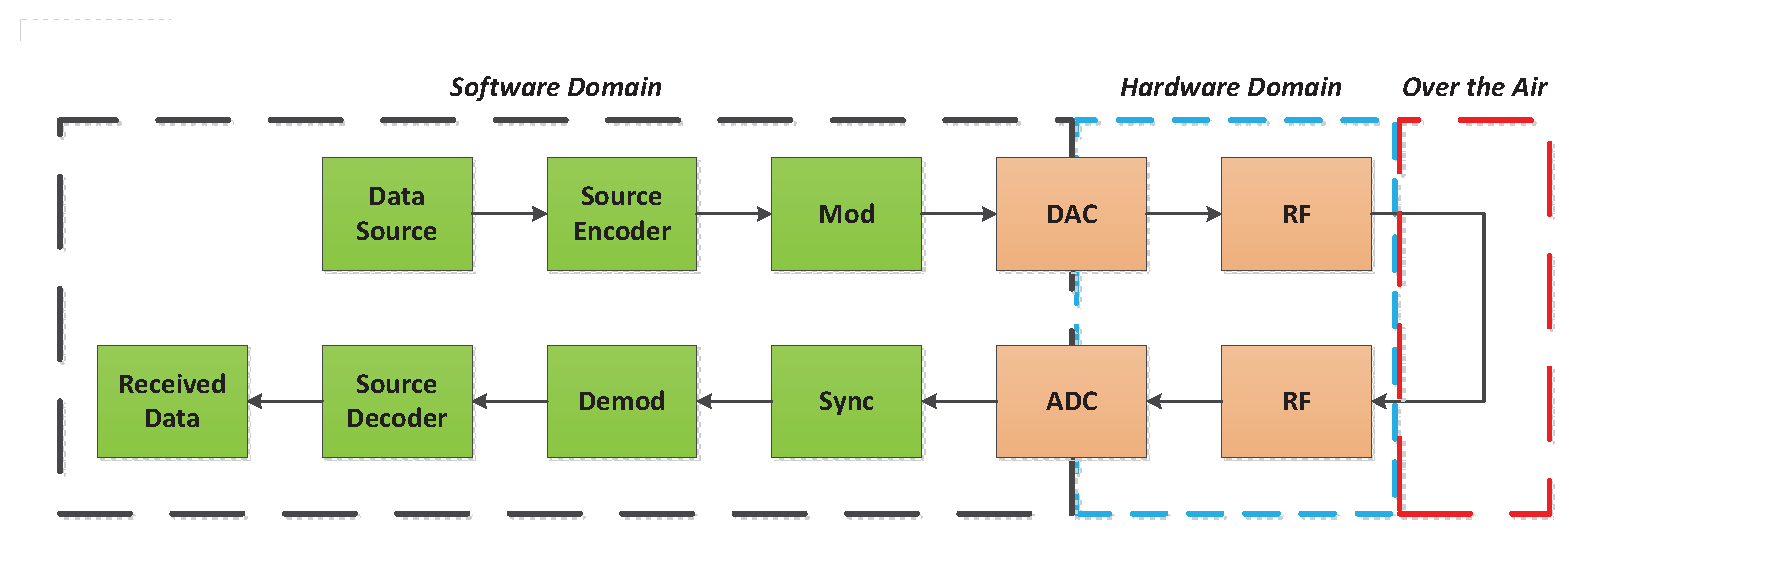
\includegraphics[scale=0.8]{sdr_overview.eps}
\caption{Software Defined Radio push all the adaptive elements and data manipulation operation into software.  The goal of SDR is to provide or define all of the radio operation in software.}
\end{figure}

Today, the main target implementations are within cellular base stations and military applications such as the JTRS project.  The JTRS or Joint Tactical Radio System, was a program of the US military to produce radios that provide flexible and inter-operable communications \cite{JTRS}. Examples of radio terminals that require support include hand-held, vehicular, airborne and dismounted radios, as well as base-stations\cite{24}.  Again, this project still has limited results and many setbacks have occurred.  Commercially, from a wide spread penetration standpoint, SDR is still many years away due to the size and cost of current devices.  The two barriers to this are speed and size.  To provide enough data throughput, modern SDRs need to quite large physically, which is a serious drawback in many applications.   Aside from these limitations, SDRs provide excellent flexibility especially in a laboratory and proof of concept environment.  Rapid prototyping is an obvious place where such radios shine, allowing massive changes without hardware modification.  To support this flexibility several software packages have been constructed around the SDR concept, allowing for aggressive prototyping.  The two examples discussed here were selected because of operability with the selected hardware, which will be discussed future in chapter 3.\\

\subsection{GNU Radio}

The first software package to be discussed by this thesis is GNU Radio.  GNU Radio provides the reconfigurable signal processing blocks that are necessary for software defined radios. GNU Radio is an open source project allowing for SDR developers to develop unique signal processing blocks and SDR systems.  GNU Radio was started in 2001, originally forked from the SpectrumWare project developed at the Massachusetts Institute of Technology \cite{spectrumware}.  Since 2001, the code base has undergone massive changes, containing almost no code from the original SpectrumWare project.  Physically the code consist of three languages Python, C++, and SWIG.  Python provides the overarching control of the system or program, while C++ provides the actual signal processing blocks and mathematics.  SWIG is a wrapper for C++ which allows Python to dynamically wrap around C++ and control or compile with it.  A diagram below better illustrates this architecture.  It is also important to mention that there as significant paradigm shifts in the community, pushing more and more code to Python rather than C++, due to its easier programming syntax and structure.\\

\begin{figure}\label{gnr_struct}
\centering
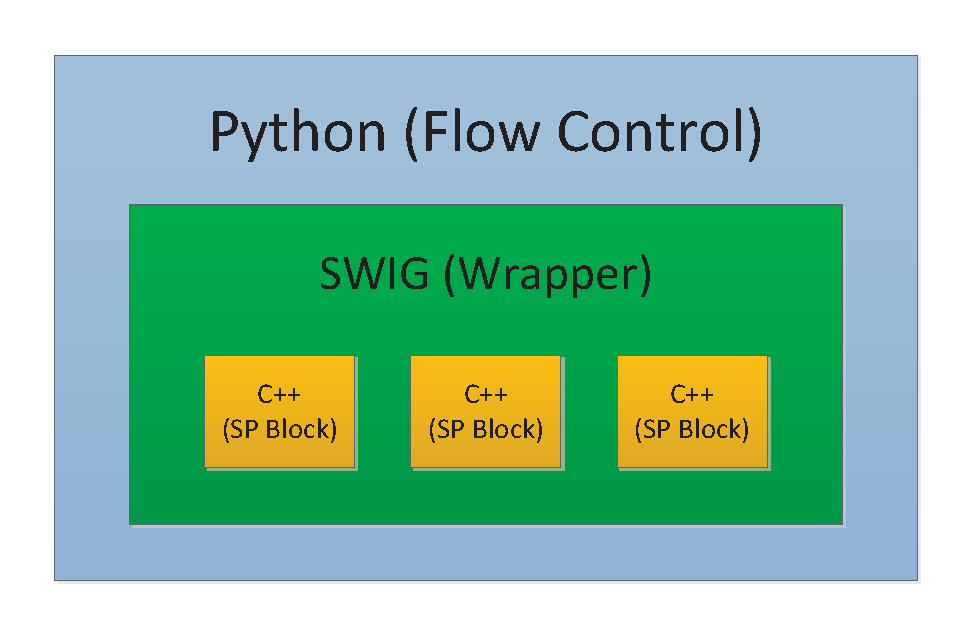
\includegraphics[scale=0.8]{gnr_outline.eps}
\caption{GNU Radio code structure based on signal processing C++ blocks and controlling, through SWIG, Python layers.}
\end{figure}

GNU Radio provides a very structured framework of flow design.  Data processing segments are extremely self contained to minimize error propagation during system debugging.  Since the software is open-source full access to all code is provide, giving low-level access to all operation within GNU Radio.  Much of the actions have been abstracted to limited the knowledge of the lower layers, but if specific actions are required for an application.  Then serious depth or knowledge is needed about the overall project's structure, which is quite overloading.\\

\subsection{MATLAB}

MATLAB is an extremely well known engineering, mathematical, biological, and financial software suite.  MATLAB provide massive data leverage and advanced communication system models and algorithm for significant data processing.  Since 2007, they have also provided hardware compliance with specific SDR platforms through their Simulink platform, and more recently within MATLAB itself \cite{matlabsdru}.  This thesis primarily utilizes the signal processing and communication system aspects of MATLAB, since MATLAB cannot fully utilize all aspects of the chosen hardware.  It is important to note under alternate constraints, MATLAB can provide adequate performance directly interfacing with hardware, especially when accessing its targeting features seen here \cite{matlabtargeting}.  Figure \ref{sdru_example} shows an example of a common MATLAB SDR model through Simulink.\\

\begin{figure}[!ht]\label{sdru_example}
\centering
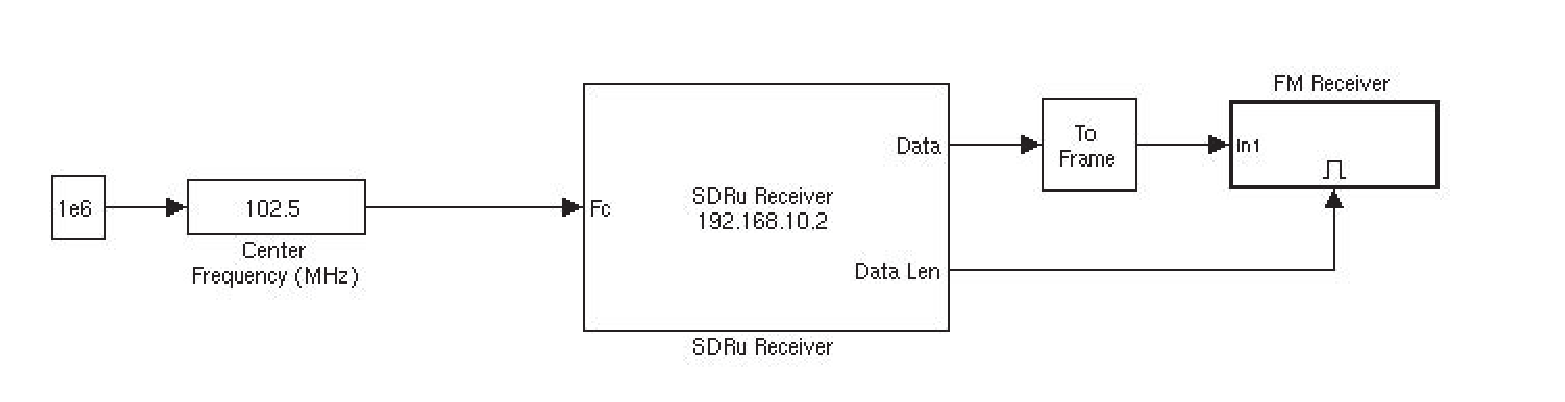
\includegraphics[scale=0.5]{sdru_example.eps}
\caption{Sample SDRU MATLAB model created in Simulink.  This model has the ability to demodulate and play FM radio stations when using a USRP device.}
\end{figure}

MATLAB provides allow connection to a USRP device through MATLAB directly of with Simulink.  The device simply acts as a real-time data source complementing their signal processing and communications toolboxes very well.  Rather than full implementations like GNUR Radio, MATLAB focuses on signal analysis rather than real-time performance.  The primary limitation is the single threaded nature of MATLAB and Simulink, which is slowly being improved upon for the SDR application.\\

\subsection{Reference Comparison}

It is important to compare GNU Radio and MATLAB, from a user's perspective they perform quite differently.  Firstly GNU Radio, is extremely fast, will the ability of sustaining the maximum throughput of the selected hardware.  GNU Radio is also multi-threaded, and while maintaining high throughput and complete background tasks on multi-core machines quite easily.  This performance has a cost, comparatively GNU Radio has an extremely learning curve and debugging can be challenging.  However if you need the performance, GNU Radio is your option, providing significantly more advanced hardware support in SDR implementations.  If data analysis is more heavily desired MATLAB is the obvious choice.  MATLAB provides easy and advanced data visualization functionality, and built in tools for analysis.  Since MATLAB does not compile itself normally, it can be much easier to debug and solve problems.  MATLAB's syntax provide similar data manipulation, especially in communication system primitives.  Therefore, it can be a rather simple choice, speed or ease of use.\\ 

\section{Summary}

This chapter outlined and examined the topics of jamming and anti-jamming techniques, and provided a foundation in communication system theory and advanced equalizer design.  Secondly it setup an understanding of Software-Defined Radio, the power of such an architecture, and examples of implementations and existing software for future designs.  Next, this thesis will consider a new anti-jamming technique and design an implementation of such a system.  After the implementation is investigated, the result of specific experiments on such an implementation will be analyzed.\\
